\chapter{Analysis Results}
\label{ch:Results}

The analysis presented in this dissertation was designed to make several measurements. As this dissertation was written alongside the first \nova~NC analysis, one primary goal of the analysis was to demonstrate the successful ability of \nova~to identify NC events and measure the ratio of observed to predicted NC events in a $3$ flavor hypothesis, $R_{NC}$.
\beq
R_{NC} \equiv \frac{ N_{Obs} - N_{Pred}^{Bkg} }{ N_{Pred}^{NC} }
\label{eq:R}
\eeq

\n The other (arguably more important) goal was to start contributing to the global data on the sterile mixing parameters by extracting measurements on the mixing angles $\theta_{24}$, $\theta_{34}$ and matrix elements $\Usqxy{\mu}{4}$ and $\Usqxy{\tau}{4}$.

Data for this analysis were collected between February $2014$ and May $2016$. For the FD, this corresponds to \pot{6.69}, or $6.05 \times 10^{20}$ full detector equivalent POT. For the ND, \pot{3.72} was collected.

The first section in this chapter describes the fitting methods used to make the mixing angle and matrix element measurements. Before presenting the results, the next two sections discuss preliminary tests to demonstrate satisfactory performance of the analysis. The final section in this chapter presents the ultimate results.

\section{Fitting Method}
\label{sec:FitMethod}

It was decided to make rate only measurements for the first \nova~NC disappearance analysis. Thus, even though the extrapolation and prediction were performed in $250\unit{MeV}$ bins of calorimetric energy, only the integrated event totals were input to the fitting framework.

Fitting was performed allowing some parameters to float, some held to current best fit values, and others set to $0$ due to insensitivity. As mentioned above, a major analysis goal was to measure $\theta_{24}$ and $\theta_{34}$, so these angles were allowed to float between $0^\circ$ and $45^\circ$. Values outside of this range are either equivalent to this range through redefinition of the angles, or already highly disfavored through previous experiments and in a region difficult for fitting due to many local minima. $\theta_{23}$ was allowed to float with a Gaussian constraint with mean $45.8^\circ$ and standard deviation $3.2^\circ$, the best fit measurement by T2K \cite{ref:T2K2015}. All of the remaining parameters were held fixed to the values listed in table \ref{tab:FitFix}.
\begin{table}[htb]
  \begin{center}
    \begin{tabular}{c c}
      \hline\hline
      Parameter & Value \\
      \hline
      $\dmxy{1}{2}$ & $7.53 \times 10^{-5}\evsq$ \\
      $\dmxy{2}{3}$ & $2.37 \times 10^{-3}\evsq$ \\
      $\sin^2 2\theta_{12}$ & $0.846$ \\
      $\sin^2 2\theta_{13}$ & $0.085$ \\
      $\theta_{14}$ & $0$ \\
      $\delta_{13}$ & $0$ \\
      $\delta_{24}$ & $0$ \\
      $\delta_{14}$ & $0$ \\
      \hline
    \end{tabular}
    \caption[Fixed Parameters and Values for Fitting]{The parameters held fixed and the values they were set at for fitting.}
    \label{tab:FitFix}
  \end{center}
\end{table}

The best fit values were found by calculating the minimum $\chi^2$ value and allowing individual systematics to float with a penalty,
\beq
\chi^2 = 2 \left( N_{Pred} - N_{Obs} + N_{Obs} \ln \frac{N_{Obs}}{N_{Pred}} \right) + \left( \frac{ \theta_{23} - \mu_{23} }{ \sigma_{23} } \right)^2 + \sum_{i=1}^{N} \left( \frac{ \sigma_i^{BF} }{\sigma_i} \right)^2,
\label{eq:Chisq}
\eeq
\n where $\mu_{23}$ and $\sigma_{23}$ are the mean and standard deviation used in the Gaussian constraint on the value of $\theta_{23}$, $\sigma_i^{BF}$ is the number of standard deviations the $i$th systematic error is shifted in the best fit, and $\sigma_i$ is one standard deviation for the $i$th systematic error. Equation \ref{eq:Chisq} is the standard formula for calculating $\chi^2$ with penalty terms, where the first term is the basic value for $\chi^2$, and the second and third terms add a unit for each shift of $\theta_{23}$ and the systematic errors by their respective variances. For one and two dimensional $\chi^2$ surfaces, the remaining angles not shown were profiled.

\section{ND Data/MC Comparisons}
\label{sec:ResultsND}

Before diving head first into the FD data, the first necessary analysis benchmark was ND data/MC comparisons. Figure \ref{fig:NDDataMCECal} shows the event energy distributions and figures \ref{fig:NDDataMCFidCont}, \ref{fig:NDDataMCNCSel}, and \ref{fig:NDDataMCCosRej} show the distributions for all of the variables used for selection discussed in chapter \ref{ch:Selection}.
\begin{figure}[htbp]
  \centering
  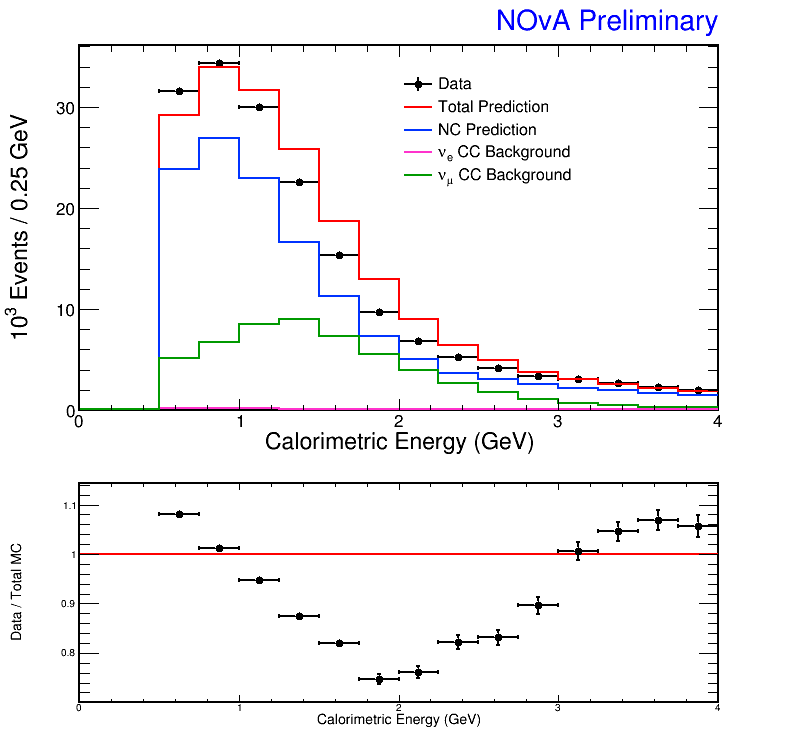
\includegraphics[width=1\textwidth]{figures/NDDataMC/ECalNusNDRat.png}
  \caption[ND Data/MC Comparison: Energy Distribution]{ND data/MC comparison of the calorimetric energy.}
  \label{fig:NDDataMCECal}
\end{figure}

\begin{figure}[htbp]
  \centering
  \begin{tabular}{c c}
    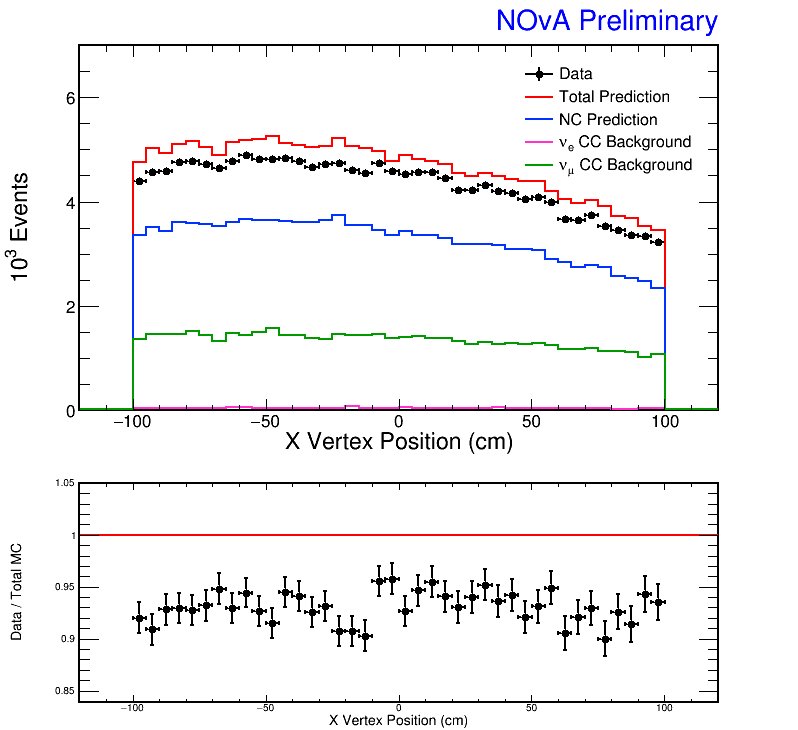
\includegraphics[width=.47\textwidth]{figures/NDDataMC/VtxXNusNDRat.png} &
    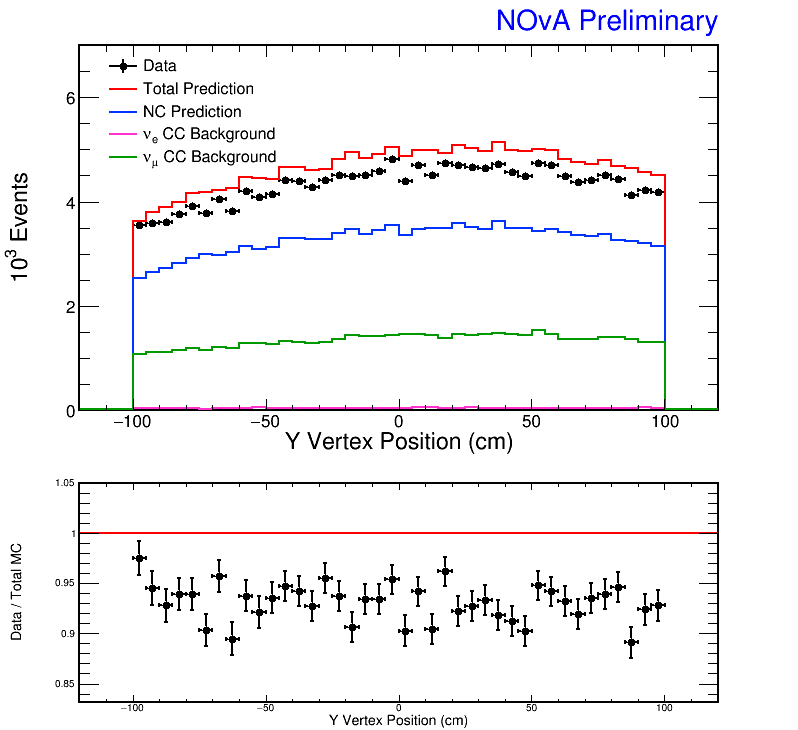
\includegraphics[width=.47\textwidth]{figures/NDDataMC/VtxYNusNDRat.png} \\
    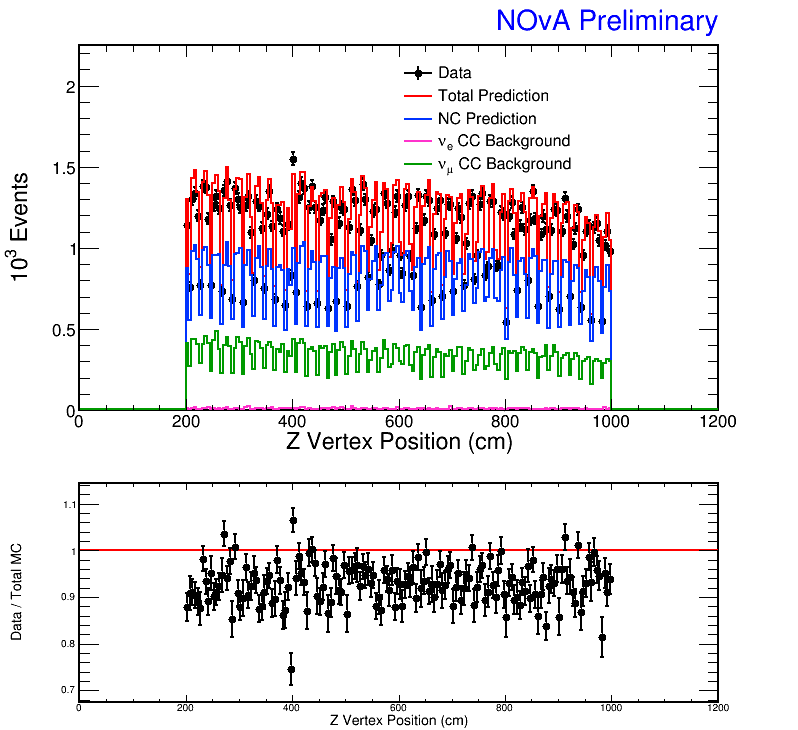
\includegraphics[width=.47\textwidth]{figures/NDDataMC/VtxZNusNDRat.png} &
    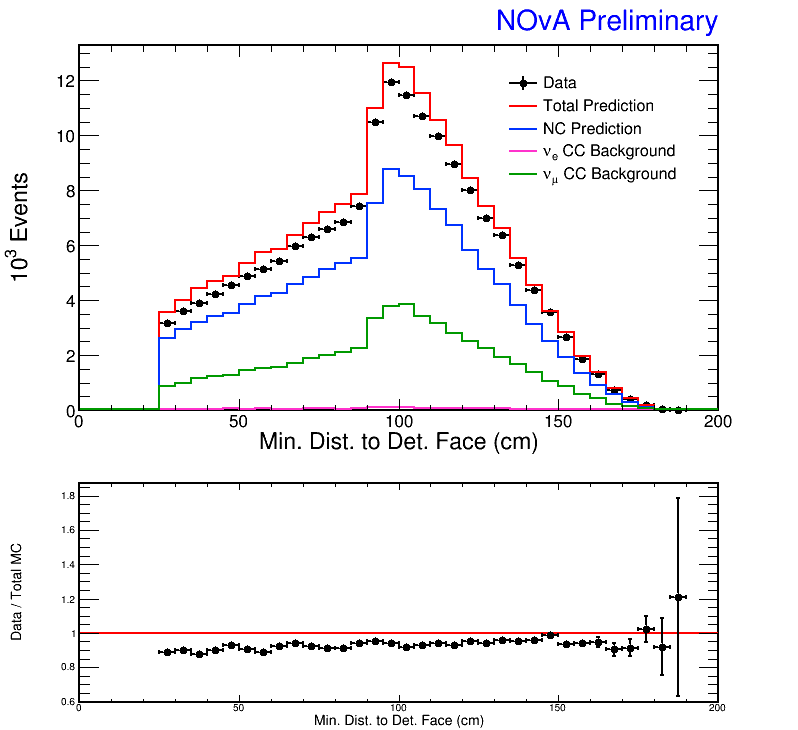
\includegraphics[width=.47\textwidth]{figures/NDDataMC/ContNusNDRat.png} \\
  \end{tabular}
  \caption[ND Data/MC Comparison: Fiducial and Containment Variable Distributions]{ND data/MC comparison of the reconstructed vertex position and containment distributions.}
  \label{fig:NDDataMCFidCont}
\end{figure}

\begin{figure}[p]
  \centering
  \begin{tabular}{c c}
    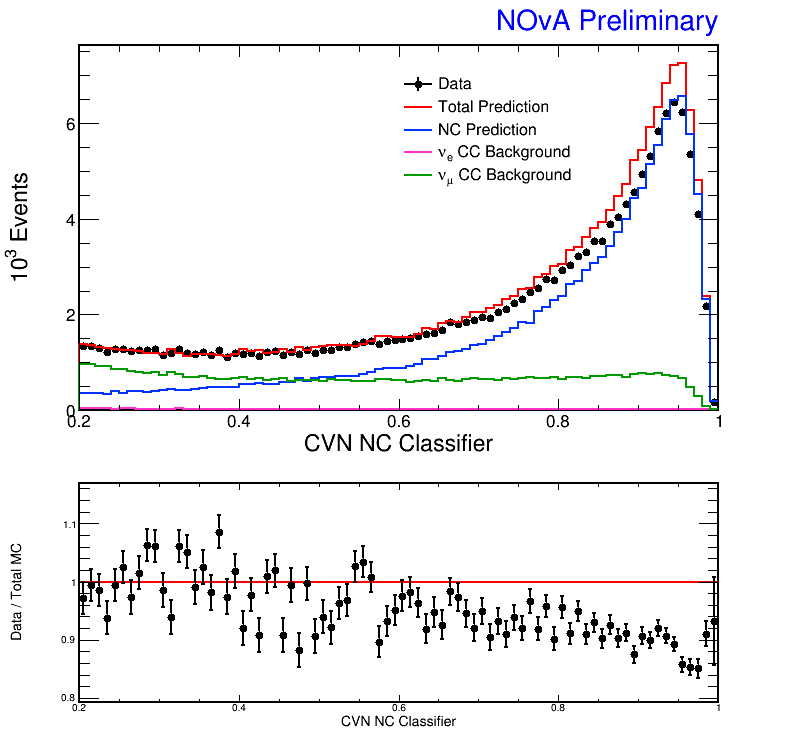
\includegraphics[width=.47\textwidth]{figures/NDDataMC/CVNNusNDRat.png} &
    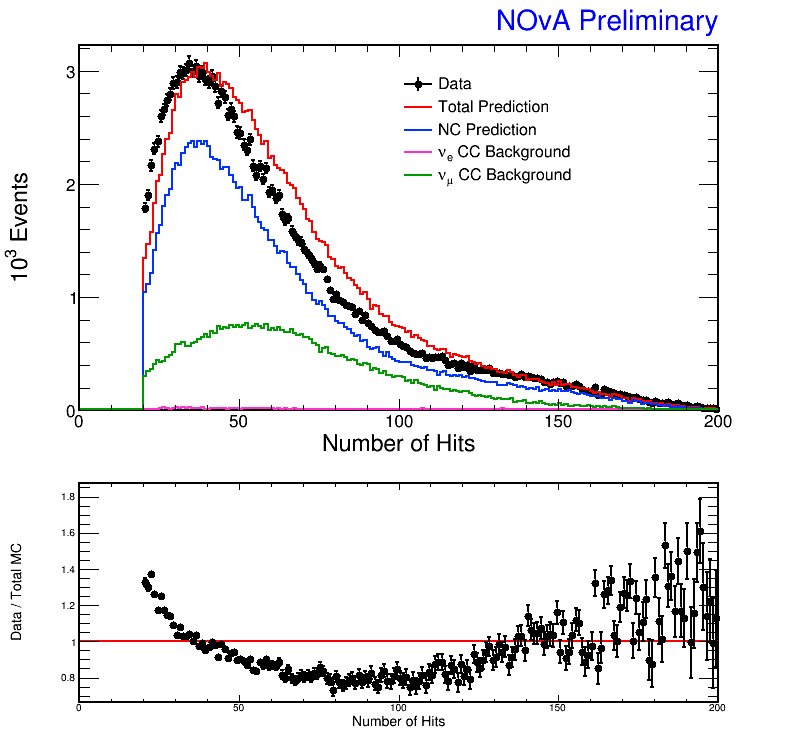
\includegraphics[width=.47\textwidth]{figures/NDDataMC/NHitNusNDRat.png} \\
  \end{tabular}
  \caption[ND Data/MC Comparison: NC Selection Variable Distributions]{ND data/MC comparison of the CVN and number of hits distributions.}
  \label{fig:NDDataMCNCSel}
\end{figure}

\begin{figure}[p]
  \centering
  \begin{tabular}{c c}
    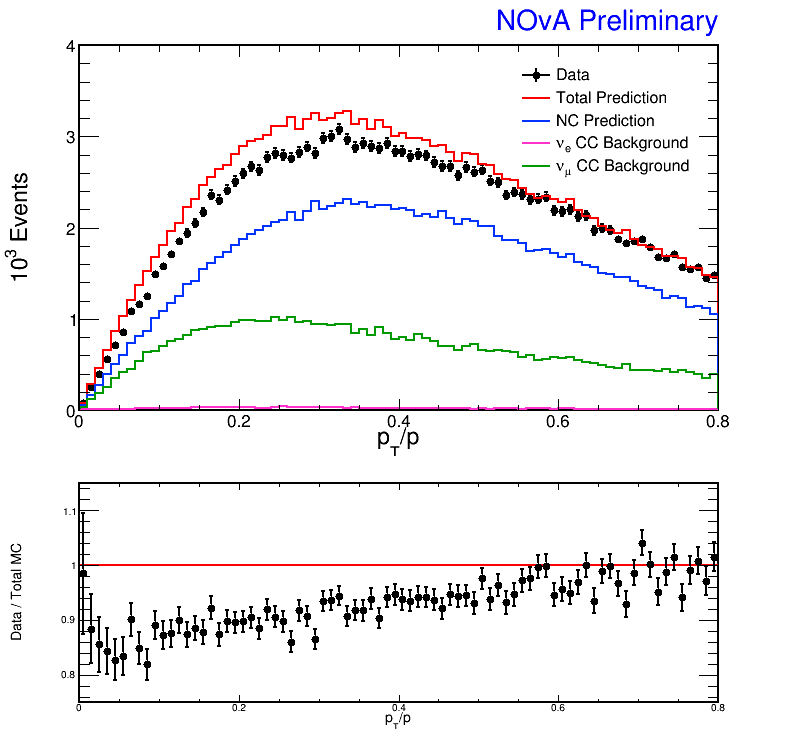
\includegraphics[width=.47\textwidth]{figures/NDDataMC/PTPNusNDRat.png} &
    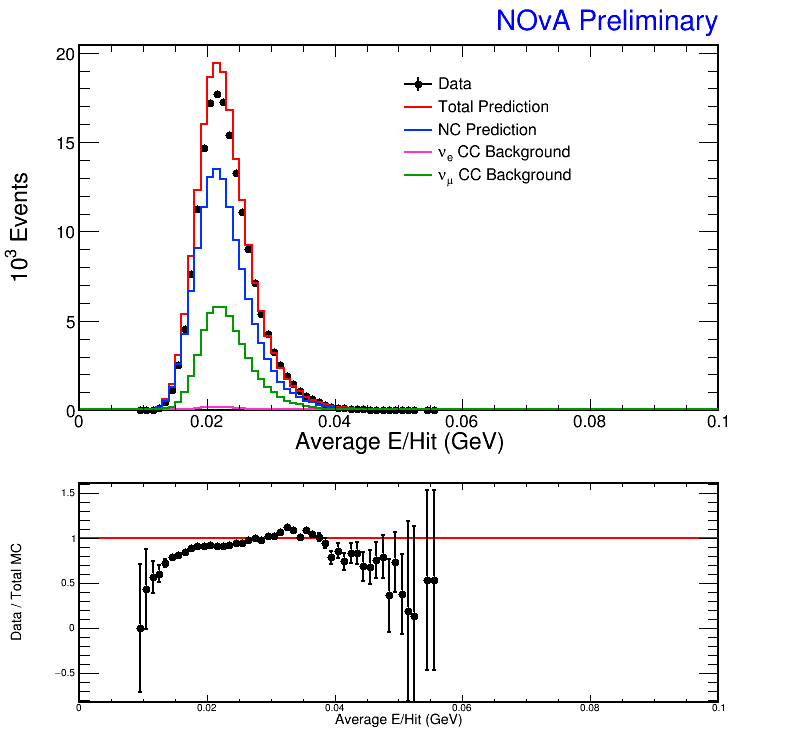
\includegraphics[width=.47\textwidth]{figures/NDDataMC/EpHNusNDRat.png} \\
  \end{tabular}
  \caption[ND Data/MC Comparison: Cosmic Rejection Variable Distribution]{ND data/MC comparison of particle transverse momentum and energy per hit distributions.}
  \label{fig:NDDataMCCosRej}
\end{figure}

\n While most of the distributions differ by at most a small normalization, a few have an apparent shift, notably the energy and number of hits distributions. Discrepancies in these particular distributions were actually expected due to a known mismodeling of NC interactions. As discussed in section \ref{sec:SimGENIE}, the newly simulated MEC event type was only added for CC events. Furthermore, there are large uncertainties in the cross sections for the resonant and DIS events. Improvements to these cross section models and inclusion of NC MEC events could largely explain the data/MC differences seen in the energy and number of hits distributions.

Two sanity checks were performed to ensure that the data/MC difference would not negatively impact the analysis. First, the ND data/MC energy distribution was shown with a full systematic error band to show the difference is covered by systematics. This was shown in figure \ref{fig:NDSystBand}. Secondly, the effect of shifting either the data or MC in relation to the other on the predicted event rate and $1$D angle sensitivities was studied. This was done by shifting the data up or the MC down by the ratio of the means of the energy distributions for MC and data, $1.39\unit{GeV} / 1.33\unit{GeV} \approx 4.5\%$ and also for a much larger shift of $10\%$. The event counts are shown in table \ref{tab:FDShift} and the angle sensitivities are shown in figure \ref{fig:1D2434Shift}. Due to the nature of a counting experiment, since the overall event rates are essentially unchanged, the effect of these rather large shifts is negligible. As a result, it was decided to take the data and MC as is and push for model improvements for future analyses.
\begin{table}[htb]
  \begin{center}
    \begin{tabular}{c c c c c c c}
      \hline\hline
      Shift & All & NC & $\numu$ CC & $\nue$ CC & Cosmic & FOM \\
      \hline
      Nominal & $83.5$ & $60.6$ & $4.6$ & $3.6$ & $14.3$ & $6.633$ \\
      Data $4.5 \%$ Up & $84.6$ & $61.0$ & $4.7$ & $3.7$ & $14.9$ & $6.634$ \\
      Data $10 \%$ Up & $86.2$ & $61.4$ & $4.9$ & $3.7$ & $15.8$ & $6.612$ \\
      MC $4.5 \%$ Down & $85.1$ & $61.8$ & $4.8$ & $3.7$ & $14.3$ & $6.702$ \\
      MC $10 \%$ Down & $87.2$ & $63.4$ & $5.2$ & $3.8$ & $14.3$ & $6.792$ \\
      \hline
    \end{tabular}
    \caption[FD Event Rates for Shifted Energy Spectra]{The number of predicted events at the FD after applying an energy shift to data or MC.}
    \label{tab:FDShift}
  \end{center}
\end{table}

\begin{figure}[htb]
  \centering
  \begin{tabular}{c c}
    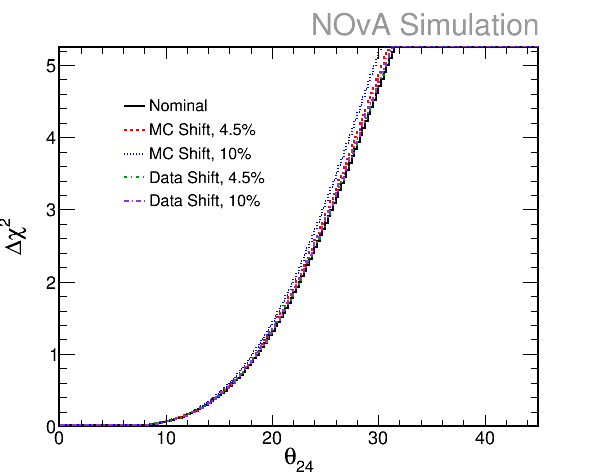
\includegraphics[width=.47\textwidth]{figures/EShift24.png} &
    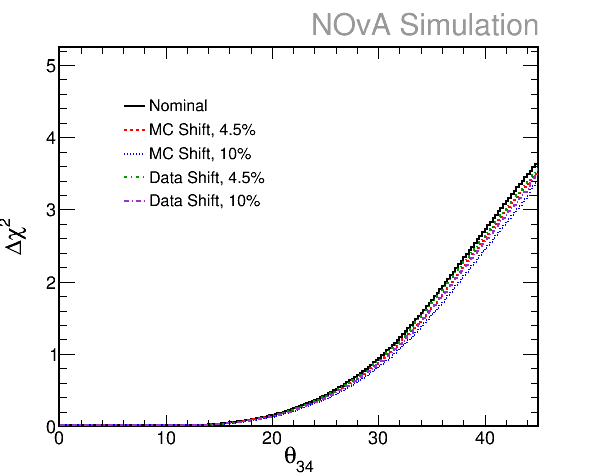
\includegraphics[width=.47\textwidth]{figures/EShift34.png} \\
  \end{tabular}
  \caption[Angle Sensitivities for Shifted Energy Spectra]{Angle sensitivities after applying an energy shift to either MC or data. Left: $\theta_{24}$, Right: $\theta_{34}$. The fits are statistics only and do not include any systematic errors.}
  \label{fig:1D2434Shift}
\end{figure}

\section{Sideband Studies}
\label{sec:Sideband}

Three different sidebands were studied to test the performance of the analysis, a high energy sideband, a low CVN sideband, and mid cosmic BDT sideband. The predicted and observed event rates for each sideband are shown in table \ref{tab:Sideband}.
\begin{table}[htbp]
  \begin{center}
    \begin{tabular}{c c c c c c c}
      \hline\hline
      Sideband & Data & Total MC & NC & $\numu$ CC & $\nue$ CC & Cosmic \\
      \hline
      High Energy & $15$ & $8.2$ & $6.5$ & $0.8$ & $0.5$ & $0.1$ \\
      Low CVN & $35$ & $32.7$ & $3.7$ & $5.5$ & $19.3$ & $4.0$ \\
      Mid BDT & $17$ & $14.5$ & $6.0$ & $0.5$ & $0.4$ & $7.5$ \\
      \hline
    \end{tabular}
    \caption[Sideband Event Rates]{The observed and predicted events at the FD for each sideband.}
    \label{tab:Sideband}
  \end{center}
\end{table}

The high energy sideband applied the standard selection and considered events between $4$ and $6\unit{GeV}$, a region chosen due to its high purity of NC events. The predicted and observed event distributions are shown in figure \ref{fig:SidebandHighE}, $8.2$ events were predicted and $15 \pm 4$ were observed in data. While the observed rate is slightly high, the low statistics means that the observation is within $2\sigma$ of the prediction. Furthermore, the discrepancy is largely driven by a single bin rather than a systematic offset. This result was thus interpreted as validation for the general analysis procedure.
\begin{figure}[htbp]
  \centering
  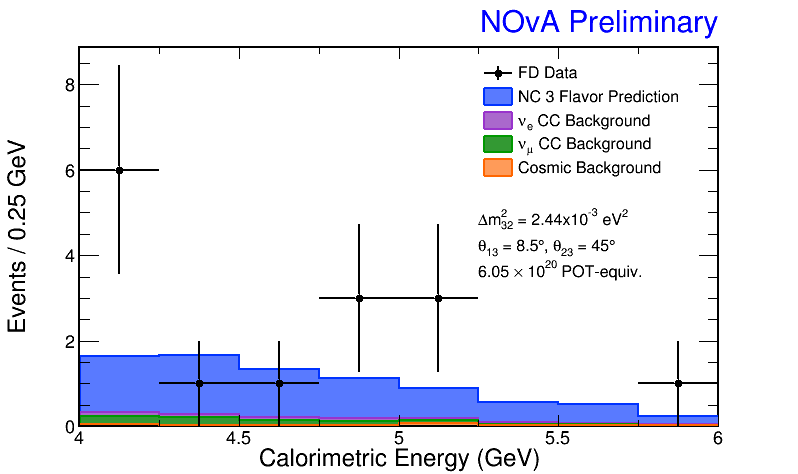
\includegraphics[width=1\textwidth]{figures/Ana01Results/FDHighECalEDataMCStack.png}
  \caption[High Energy Sideband]{The observed and predicted FD event rates for the high energy sideband.}
  \label{fig:SidebandHighE}
\end{figure}

The low CVN sideband considered events that fail the CVN cut, or those with a CVN NC score below $0.2$. This region was used as validation for the CVN selector. The predicted and observed event distributions are shown in figure \ref{fig:SidebandLowCVN}, $32.7$ events were predicted and $35 \pm 6$ were observed in data. The overall agreement in both shape and rate for this sideband provided great confidence in the performance of CVN.
\begin{figure}[htbp]
  \centering
  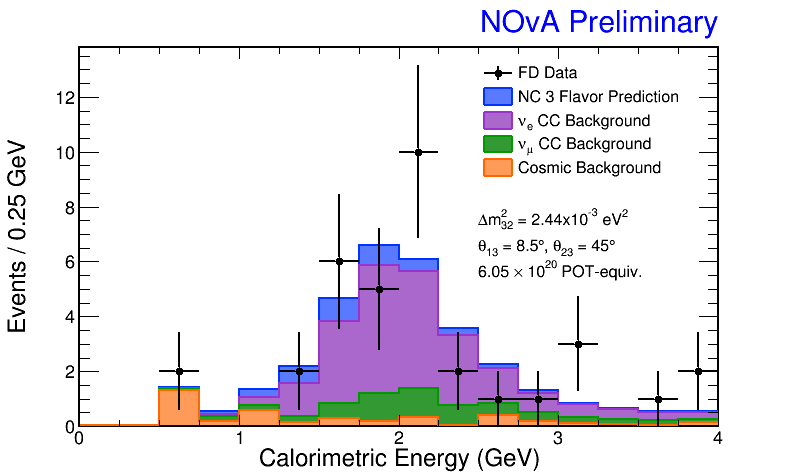
\includegraphics[width=1\textwidth]{figures/Ana01Results/FDLowCVNCalEDataMCStack.png}
  \caption[Low CVN Sideband]{The observed and predicted FD event rates for the low CVN sideband.}
  \label{fig:SidebandLowCVN}
\end{figure}

The mid cosmic BDT sideband considers events with a BDT score between $0.42$ and $0.5$, a region which fails the standard selection cuts but still has NC events. The predicted and observed event distributions are shown in figure \ref{fig:SidebandMidBDT}, $14.5$ events were predicted and $17 \pm 4$ were observed in data. This sideband also showed excellent agreement in both shape and rate, providing further validation for the general analysis procedure, and specifically for the main cosmic rejection variable.
\begin{figure}[htbp]
  \centering
  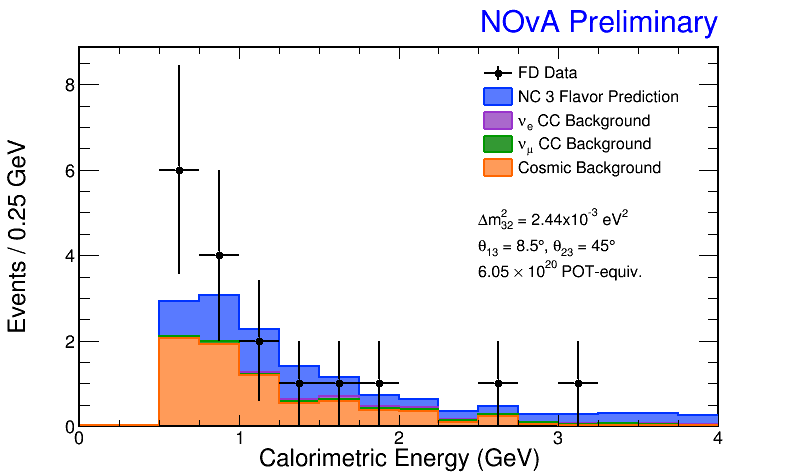
\includegraphics[width=1\textwidth]{figures/Ana01Results/FDMidBDTCalEDataMCStack.png}
  \caption[Mid Cosmic BDT Sideband]{The observed and predicted FD event rates for the mid cosmic BDT sideband.}
  \label{fig:SidebandMidBDT}
\end{figure}

\section{Results}
\label{sec:ResultsFD}

This analysis predicted that there would be $83.5 \pm 0.8 \mbox{(stat.)} ^{+10.9}_{-7.2} \mbox{(syst.)}$ NC-like events selected in the FD data. $95 \pm 9.7$ were observed, corresponding to a measurement of $R_{NC} = 1.19 \pm 0.16 \mbox{(stat.)} ^{+0.10}_{-0.14} \mbox{(syst.)}$ If active neutrinos mixed with sterile neutrinos, the number of observed events would be depleted, causing $R_{NC}$ to be less than one. Thus, the measurement of $R_{NC}$ is consistent with the no sterile mixing hypothesis.

The energy distribution of the predicted and observed events is shown in figure \ref{fig:FDDataMCECal}. The $\chi^2$ of this distribution is $23.31$ for $14$ bins, or $1.665$/bin. To better assess the understanding of the observed data, data/MC comparisons distributions were studied for many of the variables used for selection, including regions cut from the analysis. These can be seen in figures \ref{fig:FDDataMCFidCont}, \ref{fig:FDDataMCNCSel}, and \ref{fig:FDDataMCCosRej}. All of the distributions showed excellent agreement, especially within the CVN classifier. Lastly, the event vertices were well dispersed throughout the entire FD volume, as shown in figure \ref{fig:FDDataVtx}.
\begin{figure}[htbp]
  \centering
  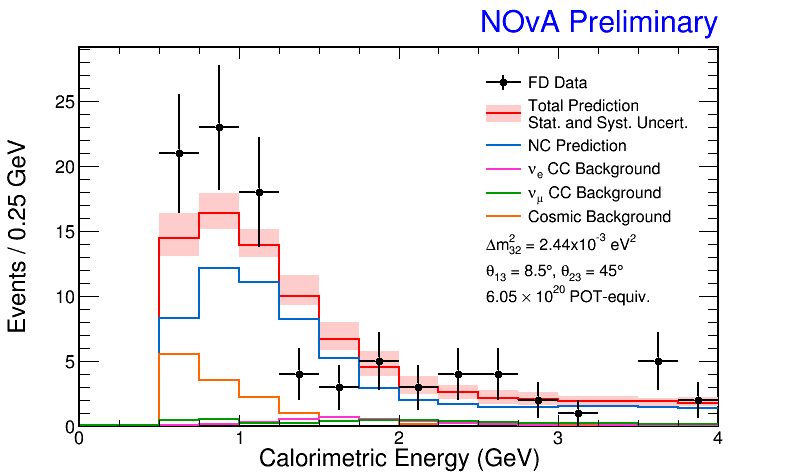
\includegraphics[width=1\textwidth]{figures/FDDataMC/cCalEFDAllStSy.png}
  \caption[FD Data and MC Energy Distribution]{Calorimetric energy distribution of events predicted and observed in the FD.}
  \label{fig:FDDataMCECal}
\end{figure}

\begin{figure}[htbp]
  \centering
  \begin{tabular}{c c}
    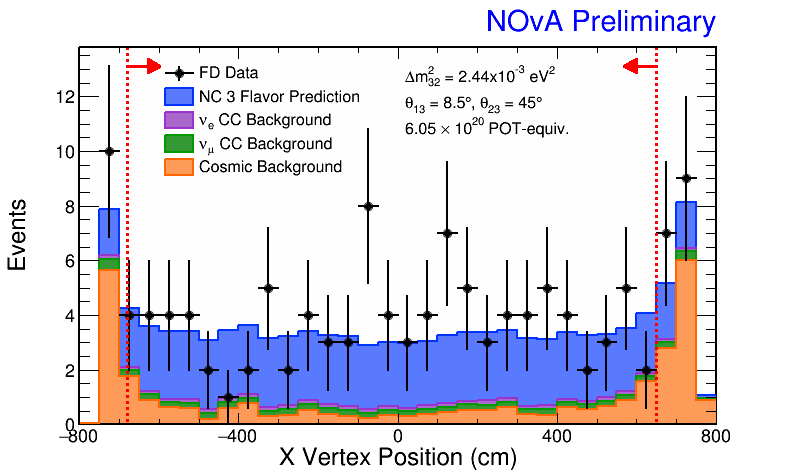
\includegraphics[width=.47\textwidth]{figures/FDDataMC/FDVtxXStack.png} &
    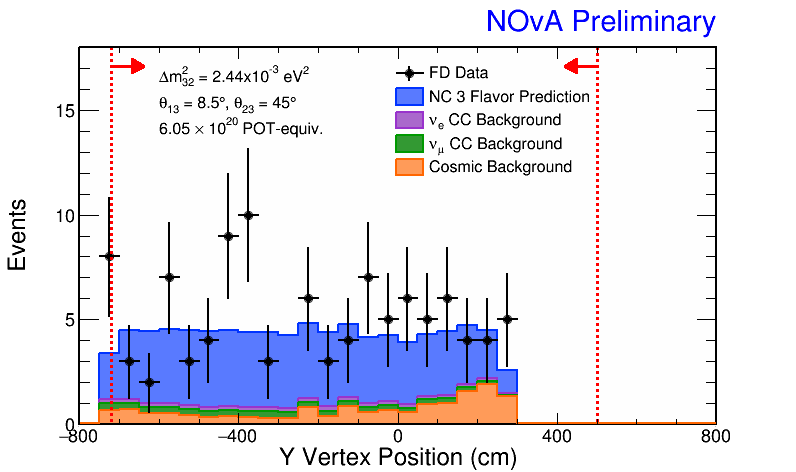
\includegraphics[width=.47\textwidth]{figures/FDDataMC/FDVtxYStack.png} \\
    \multicolumn{2}{c}{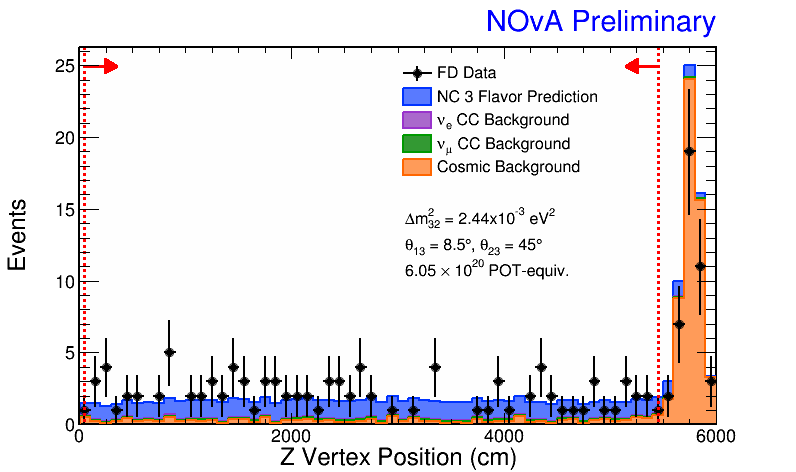
\includegraphics[width=.47\textwidth]{figures/FDDataMC/FDVtxZStack.png}} \\
  \end{tabular}
  \caption[FD Data/MC Comparison: Fiducial Variable Distributions]{FD data/MC comparison of the reconstructed vertex position distributions. The dashed lines and arrows indicate the regions kept for the analysis.}
  \label{fig:FDDataMCFidCont}
\end{figure}

\begin{figure}[htbp]
  \centering
  \begin{tabular}{c c}
    \multicolumn{2}{c}{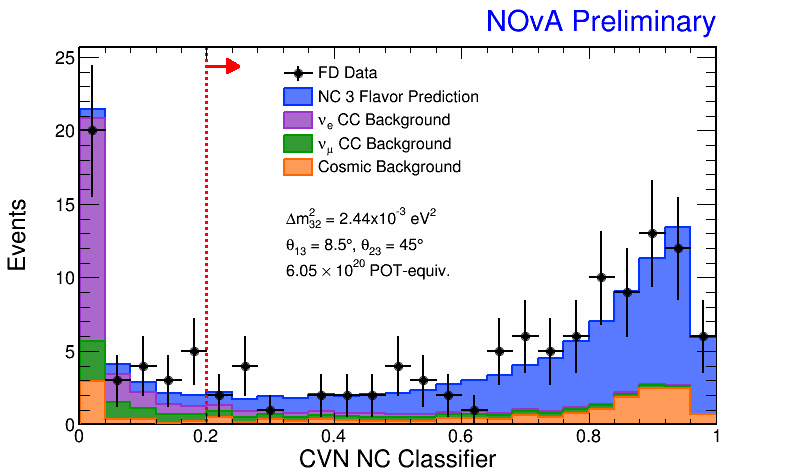
\includegraphics[width=.47\textwidth]{figures/FDDataMC/FDCVNStack.png}} \\
  \end{tabular}
  \caption[FD Data/MC Comparison: CVN Distribution]{FD data/MC comparison of the CVN distribution. The dashed line and arrow indicate the region kept for the analysis.}
  \label{fig:FDDataMCNCSel}
\end{figure}

\begin{figure}[htbp]
  \centering
  \begin{tabular}{c c}
    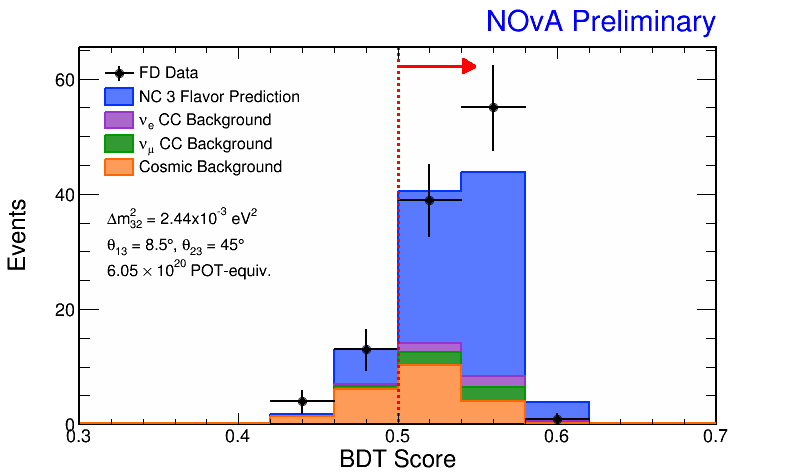
\includegraphics[width=.47\textwidth]{figures/FDDataMC/FDCosBDTStack.png} &
    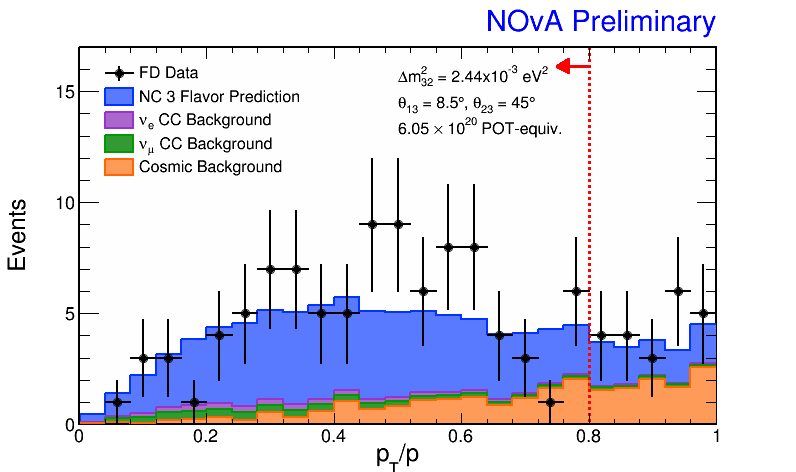
\includegraphics[width=.47\textwidth]{figures/FDDataMC/FDPTPStack.png} \\
    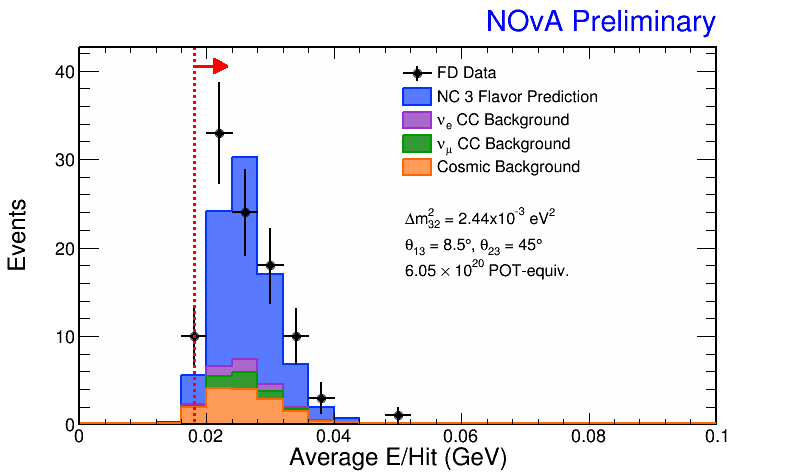
\includegraphics[width=.47\textwidth]{figures/FDDataMC/FDEperHitStack.png} &
    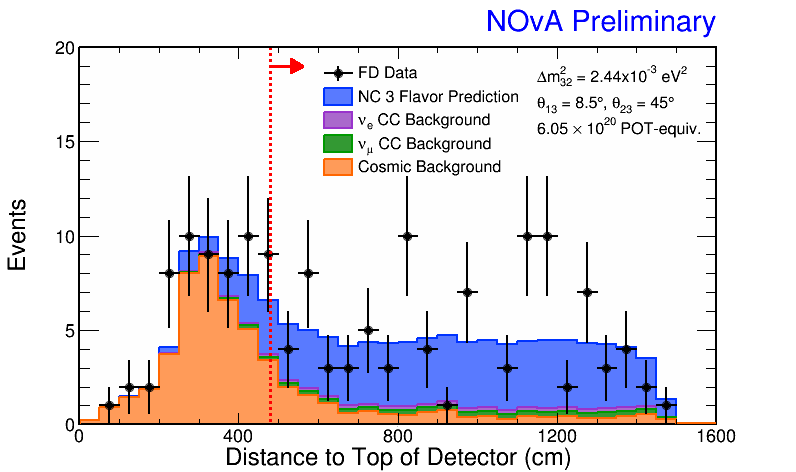
\includegraphics[width=.47\textwidth]{figures/FDDataMC/FDDistTopStack.png} \\
  \end{tabular}
  \caption[FD Data/MC Comparison: Cosmic Rejection Variable Distributions]{FD data/MC comparisons of the variables used for cosmic rejection. The dashed lines and arrows indicate the regions kept for the analysis.}
  \label{fig:FDDataMCCosRej}
\end{figure}

\begin{figure}[p]
  \centering
  \begin{tabular}{c}
    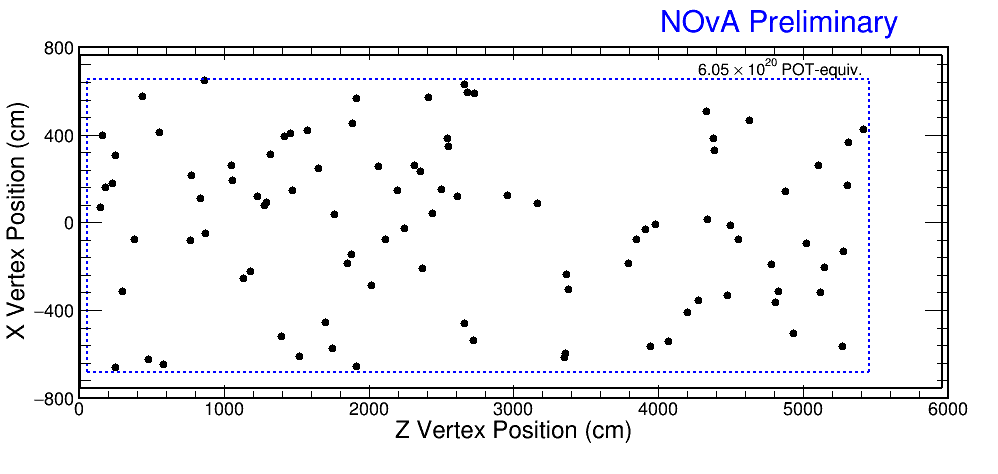
\includegraphics[width=.8\textwidth]{figures/VtxDistFDXZ.png} \\
    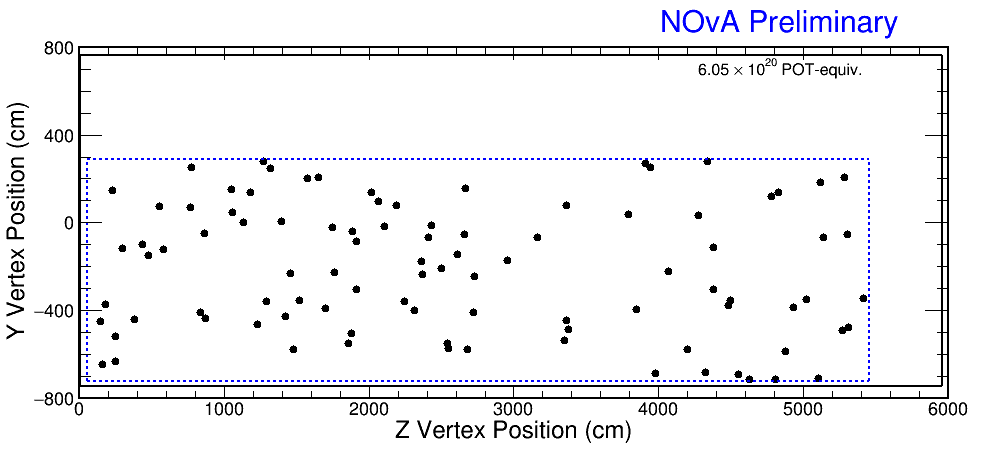
\includegraphics[width=.8\textwidth]{figures/VtxDistFDYZ.png} \\
    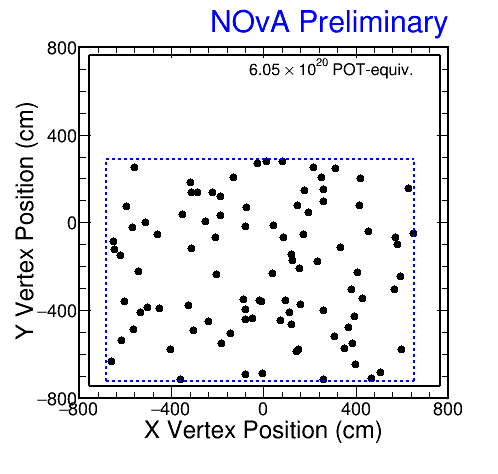
\includegraphics[width=.4\textwidth]{figures/VtxDistFDXY.png} \\
  \end{tabular}
  \caption[FD Data Vertex Distributions]{Distributions of the selected data event vertices in the detector. The solid black outline shows the full detector volume; the dashed blue line shows the fiducial and contained region. Top: XZ view. Middle: YZ view. Bottom: XY view.}
  \label{fig:FDDataVtx}
\end{figure}

Oscillation parameter measurements were extracted from a fit to the data, using the methods described in section \ref{sec:FitMethod}. The two dimensional $68\%$ and $90\%$ confidence levels are shown in figure \ref{fig:Fit2D}. One dimensional slices of $\theta_{24}$ and $\theta_{34}$ were constructed from the full fit by profiling over the remaining angles and can be seen in figure \ref{fig:Fit1D}. The best fit values were within an arc second of $0^\circ$, and from the one dimensional slices the mixing angles were limited to $\theta_{34} < 35^\circ$ and $\theta_{24} < 21^\circ$ at $90\%$ confidence. The $\theta_{34}$ limit is already competitive with the MINOS $2011$ result \cite{ref:MINOSSterile}, also shown in figure \ref{fig:Fit2D}.
\begin{figure}[htbp]
  \centering
  \begin{tabular}{c c}
    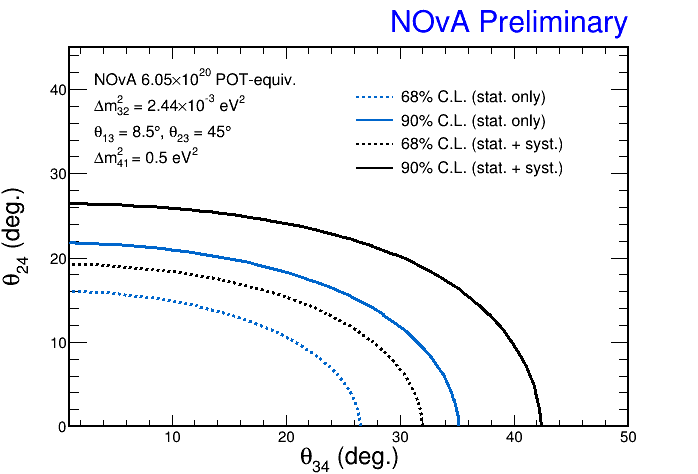
\includegraphics[width=.47\textwidth]{figures/Fits/2D3424.png} &
    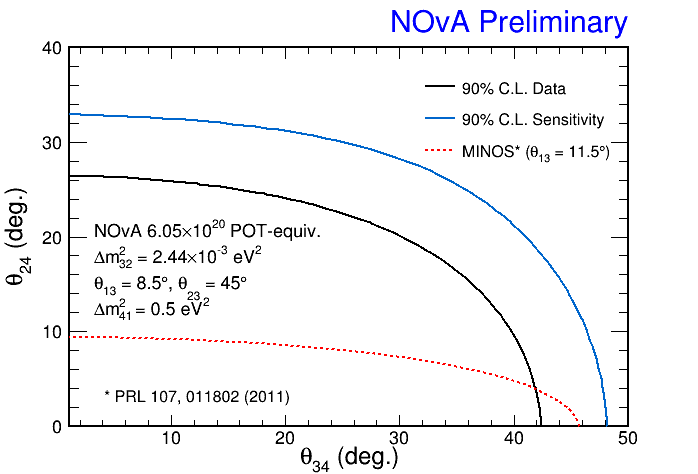
\includegraphics[width=.47\textwidth]{figures/Fits/2D3424_MINOS.png} \\
  \end{tabular}
  \caption[Two Dimensional $\theta_{34}$ vs $\theta_{24}$ Contours]{Two dimensional contours of $\theta_{34}$ vs $\theta_{24}$. The left figure shows the $68\%$ and $90\%$ confidence limits. The right figure shows the $90\%$ confidence limit with a comparison to the MINOS $2011$ results \cite{ref:MINOSSterile}.}
  \label{fig:Fit2D}
\end{figure}

\begin{figure}[htbp]
  \centering
  \begin{tabular}{c c}
    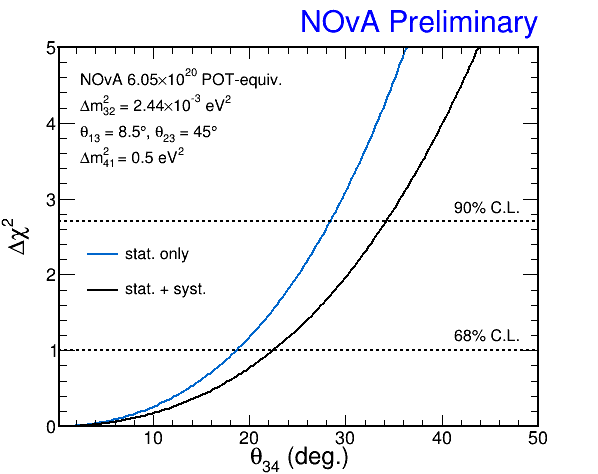
\includegraphics[width=.47\textwidth]{figures/Fits/1DTh34.png} &
    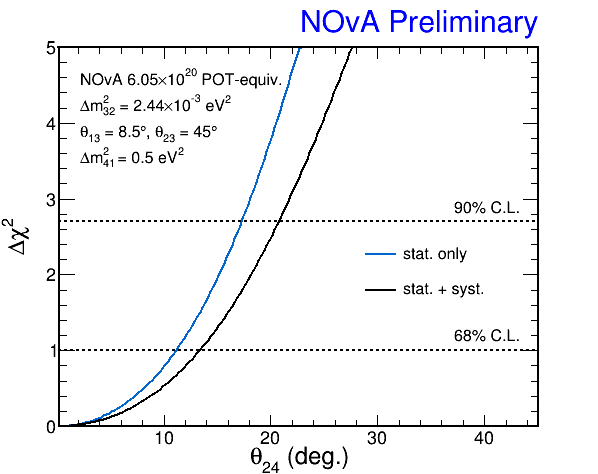
\includegraphics[width=.47\textwidth]{figures/Fits/1DTh24.png} \\
  \end{tabular}
  \caption[One Dimensional $\theta_{34}$ and $\theta_{24}$ Slices]{One dimensional slices of $\theta_{34}$ and $\theta_{24}$. These distributions were constructed by profiling over the remaining angles from the fit. Left: $\theta_{34}$. Right: $\theta_{24}$.}
  \label{fig:Fit1D}
\end{figure}

The data were also analyzed using a Feldman-Cousins (FC) statistical correction \cite{ref:FC}. The basic pre\-mise of this technique is to extract confidence intervals from an ordered likelihood ratio, instead of directly from $\Delta\chi^2$ values. The FC method performs particularly well near physical boundaries, such as angles close to maximum or minimum. The likelihood ratio, $R$, is calculated from
\beq
R_{i} = P\left( x_i | x_e\left(\vec{\theta}\right) \right) / P\left( x_i | x_e\left(\vec{\theta}_{BF}\right) \right),
\label{eq:FCRank}
\eeq

\n where $P$ is the Poisson probability of observing $x_i$ events based on an expectation of $x_e$, and $x_e$ is a function of the parameters $\vec{\theta}$. Holding to a fixed $\vec{\theta}$, all $R_i$ are calculated and ordered from highest to lowest. The exclusion significance, $c$, of $\vec{\theta}$ is then calculated from
\beq
c = \sum_{i | R_i = R_{Max}}^{i | R_i = R_{Data}} P\left(x_i | x_e\left(\vec{\theta}\right)\right).
\label{eq:FCConf}
\eeq

\n In practice, all $R_i$ are not necessary, which is important as $x_i$ goes from $0$ to infinity. Instead, two facts are used to limit the number of calculations. First, the max rank is found using the fact that the Poisson probability peaks when the observed rate matches the mean. Second, since the probability summation stops when $R_i < R_{Data}$, the $R_i$ are calculated moving outward from $x_{Max}$ until this condition is met.

Nuisance parameters, including $\theta_{23}$ and the systematics, are handled by including and profiling them in equations \ref{eq:FCRank} and \ref{eq:FCConf} \cite{ref:FCNotes}. Specifically,
\beq
R_{i} = P\left( x_i | x_e\left(\vec{\theta}, \vec{\lambda}_{BF(Data)}\right) \right) / P\left( x_i | x_e\left(\vec{\theta}_{BF}, \vec{\lambda}_{BF}\right) \right),
\label{eq:FCRankLambda}
\eeq

\n where in the numerator, $\vec{\lambda}_{BF(Data)}$ is found by fitting to the actual data, and $\vec{\lambda}_{BF}$ in the denominator is calculated by fitting to the possible observation $x_i$. In other words,
\beq
\vec{\lambda}_{BF(Data)} = \vec{\lambda} | \chi^2\left(x_{Data}, \vec{\theta}, \vec{\lambda}\right) = \chi^2_{Min}\left(x_{Data}, \vec{\theta}\right),
\label{eq:FCLambdaNum}
\eeq
\beq
\left(\vec{\theta}_{BF}, \vec{\lambda}_{BF}\right) = \left(\vec{\theta}, \vec{\lambda}\right) | \chi^2\left(x_i, \vec{\theta}, \vec{\lambda}\right) = \chi^2_{Min}(x_i).
\label{eq:FCLambdaDen}
\eeq

\n The confidence interval is calculated using the best fit of the nuisance parameters to the data,
\beq
c = \sum_{i | R_i = R_{Max}}^{i | R_i = R_{Data}} P\left(x_i | x_e\left(\vec{\theta}, \vec{\lambda}_{BF(Data)}\right)\right),
\label{eq:FCConfLambda}
\eeq

\n where $R_i$ is that which includes the nuisance parameters calculated from equation \ref{eq:FCRankLambda}.

The results of the FC corrections are shown in figure \ref{fig:Fit2DFC}, which shows the significance surface and compares the FC corrected $68\%$ and $90\%$ contours to their uncorrected counterparts. The massive improvement is largely an artifact of the assumed numbers of degrees of freedom (DOF). The uncorrected curves were constructed varying $\theta_{34}$ and $\theta_{24}$ in equation \ref{eq:Chisq}, generating a $\Delta\chi^2$, and interpreting the result assuming a separate DOF for each angle. For $2$ DOF, the $68\%$ contour was thus calculated where $\Delta\chi^2 = 2.30$, and the $90\%$ contour at $\Delta\chi^2 = 4.61$. Given that the fits had a single measured number as input, using $2$ DOFs was dubious, though it only resulted in an overly conservative limit. On the other hand, the FC corrected contour only considered a single DOF by construction.
\begin{figure}[htbp]
  \centering
  \begin{tabular}{c c}
    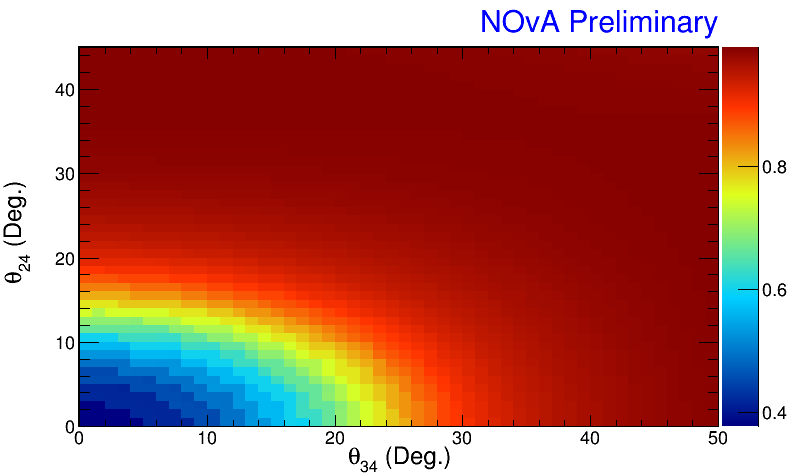
\includegraphics[width=.47\textwidth]{figures/Fits/cFCSig.png} &
    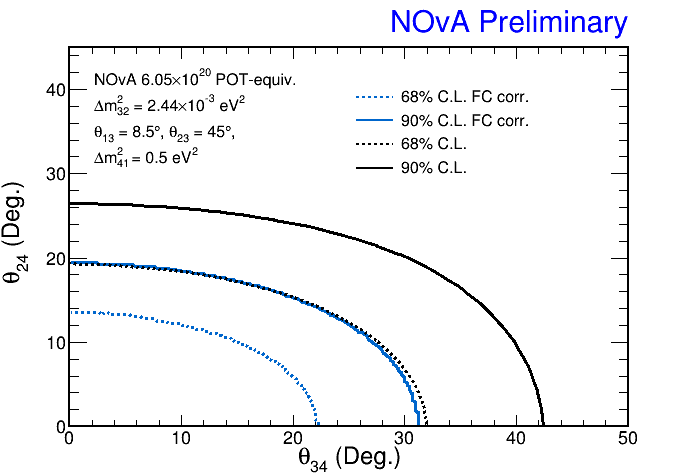
\includegraphics[width=.47\textwidth]{figures/Fits/2D3424FC.png} \\
  \end{tabular}
  \caption[FC Corrected Significance Surface and $68\%$ and $90\%$ Contours]{Left: the FC corrected significance surface. The $(\theta_{34}, \theta_{24})$ values are included in a $c\%$ confidence interval if the significance value is $\leq c$. Right: the $68\%$ and $90\%$ FC contours as compared to the uncorrected contours.}
  \label{fig:Fit2DFC}
\end{figure}

The two dimensional surface was profiled to create one dimensional slices of the two angles. These are shown in figure \ref{fig:Fit1DFC} with a comparison to the uncorrected versions. Here, the results are much more consistent, as the uncorrected one dimensional slices only show a single DOF.
\begin{figure}[htbp]
  \centering
  \begin{tabular}{c c}
    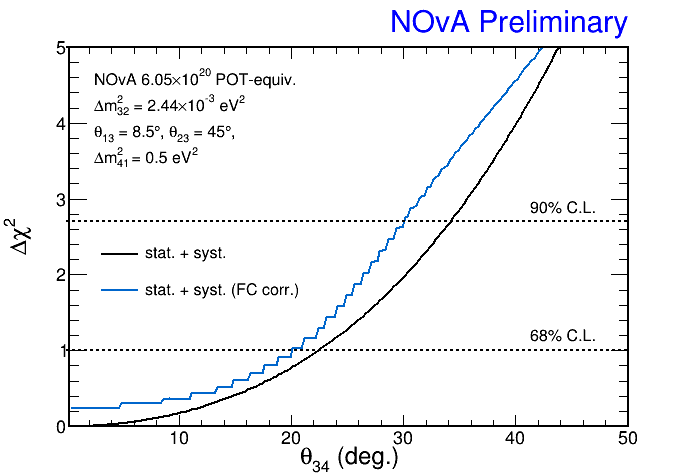
\includegraphics[width=.47\textwidth]{figures/Fits/1DTh34FC.png} &
    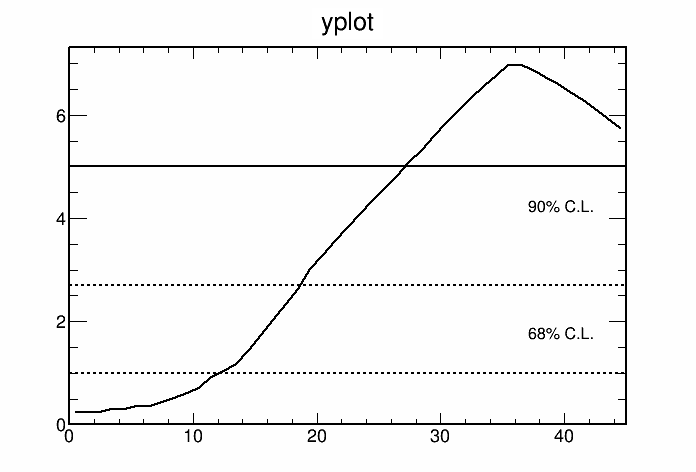
\includegraphics[width=.47\textwidth]{figures/Fits/1DTh24FC.png} \\
  \end{tabular}
  \caption[FC Corrected One Dimensional $\theta_{34}$ and $\theta_{24}$ Slices]{One dimensional slices of $\theta_{34}$ and $\theta_{24}$, with the uncorrected slice in black and the FC corrected slice in blue. Left: $\theta_{34}$. Right: $\theta_{24}$.}
  \label{fig:Fit1DFC}
\end{figure}

The final results of the analysis, based on the FC corrected surface, placed upper limits on the mixing angles and matrix elements. The sterile mixing angle limits were measured at $\theta_{34} < 30^\circ$ and $\theta_{24} < 19^\circ$ at the $90\%$ confidence level. These values were converted into measurements of the matrix elements via
\beqa
\Usqxy{\mu}{4} &=& \sin^2\theta_{24} \nonumber\\
\Usqxy{\tau}{4} &=& \cos^2\theta_{24} \sin^2\theta_{34} \label{eq:MatrixResults}
\eeqa

\n where $\theta_{14} = 0$ is assumed. The limits on the matrix elements were measured to be $\Usqxy{\mu}{4} < 0.10$ and $\Usqxy{\tau}{4} < 0.25$ at the $90\%$ confidence level.

%The actual FC procedure was to run many pseudo-experiments in each bin of $\vec{\theta} \equiv (\theta_{34}, \theta_{24})$, construct a `critical value surface' from the results, and compare the $\chi^2$ of the actual data to the critical surface.
%
%For a given bin in $\vec{\theta}$ space, $2500$ pseudo-experiments were run by randomly picking a `true' $\vec{\theta}$ from within the bin with uniform probability. A mock data spectrum was created by calculating a MC spectrum from the chosen $\vec{\theta}$ and Poisson varying each bin. Two fits were then performed to the mock data using equation \ref{eq:Chisq} with the systematic errors seeded randomly from a Gaussian with mean $0$ and standard deviation $1$. One fit allowed $\vec{\theta}$ to float as normal to calculate $\chi^2_{Best}$, and the other fit used the fixed, true $\vec{\theta}$ to calculate $\chi^2_{True}$. All of the pseudo-experiment results were then ordered by $\Delta\chi^2_{FC} = \chi^2_{True} - \chi^2_{Best}$, and this process was repeated for each bin in $\vec{\theta}$ space.
%
%Critical value surfaces were next constructed from the results of the pseudo-experiments with each surface corresponding to a particular confidence level, $c$, where $0 < c < 1$. For each bin in $\vec{\theta}$ space, a $\Delta\chi^2_c$ was calculated such that $c\%$ of the pseudo-experiments satisfied $\Delta\chi^2_{FC} < \Delta\chi^2_c$ and the remaining $(1-c)\%$ satisfied $\Delta\chi^2_{FC} > \Delta\chi^2_{c}$. This set of $\{\Delta\chi^2_c\}$ represents the $\chi^2$ values that correspond to the confidence level $c$, much like $\chi^2 = 2.71$ represents a $90\%$ confidence level for a Gaussian distributed random variable. The $\chi^2$ surface from the data was then compared to the critical value surface. In the Gaussian analogy, the $90\%$ confidence interval is constructed by including the set of parameters with $\chi^2_{Data} < 2.71$. Similarly, the FC corrected $c$ confidence level was constructed from the set of parameters, $\vec{\theta}$, such that $\chi^2_{Data} < \chi^2_c$.
%
%The critical value surfaces for the $68\%$ and $90\%$ confidence levels are shown in figure \ref{fig:FCCritical}. Figure \ref{fig:Fit2DFC} shows the two dimensional FC corrected contour with a comparison to the conventional contour.
%\begin{figure}[htbp]
%  \centering
%  \begin{tabular}{c c}
%    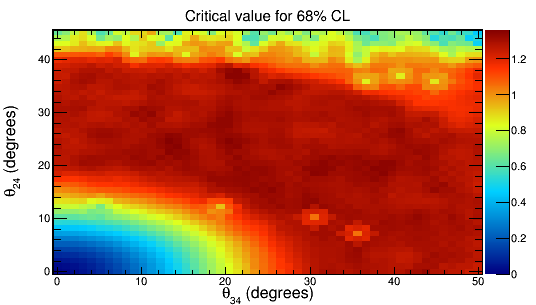
\includegraphics[width=.47\textwidth]{figures/Fits/FC68Smooth.png} &
%    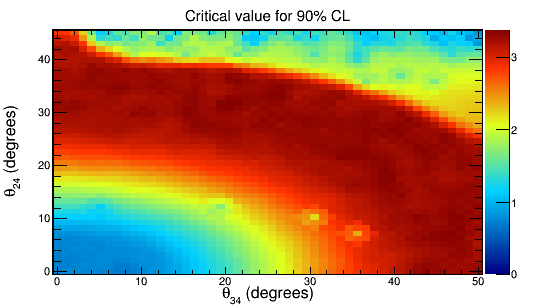
\includegraphics[width=.47\textwidth]{figures/Fits/FC90Smooth.png} \\
%  \end{tabular}
%  \caption[FC $68\%$ and $90\%$ Critical Surfaces for $\theta_{34}$ vs $\theta_{24}$]{FC $68\%$ (left) and $90\%$ (right) critical value surfaces for $\theta_{34}$ vs $\theta_{24}$. These surfaces had a standard smoothing algorithm applied to them.}
%  \label{fig:FCCritical}
%\end{figure}
%
%\begin{figure}[htbp]
%  \centering
%  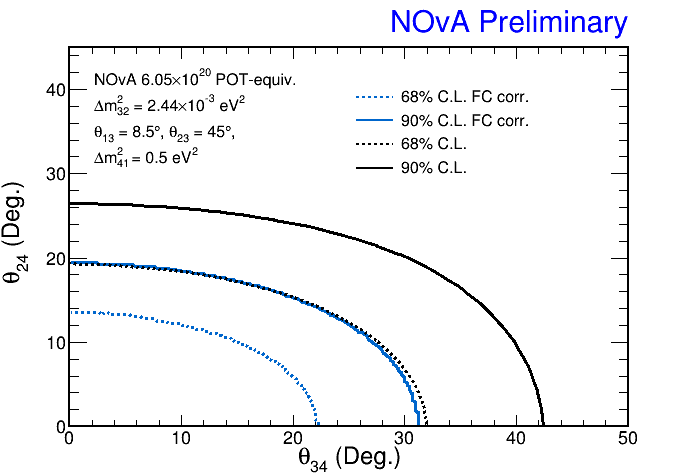
\includegraphics[width=.47\textwidth]{figures/Fits/2D3424FC.png} \\
%  \caption[FC Corrected Two Dimensional $\theta_{34}$ vs $\theta_{24}$ Contours]{Two dimensional contours of $\theta_{34}$ vs $\theta_{24}$. The blue curves show the FC corrected contours, and the black curves are the standard calculated curves from figure \ref{fig:Fit2D} shown for comparison.}
%  \label{fig:Fit2DFC}
%\end{figure}